\section{Design \& Architecture}\label{sec:Design}

\subsection{Key Design Decisions}

Taking into account the repetitive nature of the calculations,
and the need for shorthand notations we very rapidly converged
on four initial design decisions:
\begin{enumerate}
  \item No parsers! All calculation objects are written
  directly in Haskell.
  \item We would keep the expression and predicate datatype declarations
   very simple, with only equality being singled out.
  \item We would need to have a good way to pretty-print long predicates
    that made it easy to see their overall structure
  \item We would rely on a dictionary based system to
    make it easy to customise how specific constructs
    were to be handled.
\end{enumerate}
From our experience with the \UTP2 theorem-prover we also decided
the following regarding the calculation steps that would be supported:
\begin{itemize}
  \item
    We would not support full  propositional calculus
    or theories of numbers or sets.
    Instead we would support the use of hard-coded relevant laws,
    typically derived from  a handwritten proof.
  \item
    We would avoid, at all costs,
    any use of quantifiers or binding constructs.
  \item
    The calculator user interface would be very simple,
    supporting a few high level commands such as ``simplify''
    or ``reduce''.
    In particular,
    no facility would be provided for the user to identify
    the relevant sub-part of the current goal to which any operation
    should be applied.
\end{itemize}

\subsection{The Calculator REPL}

The way the calculator is designed to be used is
that a function implementing a calculator Read-Execute-Print-Loop (REPL)
is given a dictionary and starting predicate as inputs.
It then offers the user the opportunity to invoke various
commands to perform calculation steps.
The user can then indicate when they are finished,
at which point the calculator function returns
a data-structure that logs the complete calculation outcome.

Calculator commands include an ability to undo previous steps ('\texttt{u}'),
request help ('\texttt{?}'),
and to signal an exit from the calculator ('\texttt{x}').
However,
of most interest are the five calculation commands.
The first is a global simplify command ('\texttt{s}'),
that scans the entire predicate from the bottom-up
looking for simplifiers for each composite and applying them.
Simplifiers are captured as \texttt{eval} or \texttt{prsimp} components
in dictionary entries.

The other four commands work by searching top-down, depth-first for
the first sub-component for which the relevant dictionary calculator
function returns a changed result.
Here is where we have a reduced degree of control,
which simplifies the REPL dramatically,
but turns out to be strikingly effective in practice.
This is because these kinds of semantic ``smoke-test'' calculations
tend to go in phases: expand all definitions; simplify; reduce; simplify;
perhaps unroll a loop a bit; etc...
\begin{description}
  \item[Defn. Expand ('\texttt{d}')]
    Find the first predicate changed by applying its
     \texttt{pdefn} dictionary entry, which should unfold its definition.
  \item[Law Reduce ('\texttt{r}')]
    Find the first predicate transformed by a function
    in the \texttt{reduce} list of the \texttt{LawEntry} indexed
     by the string \texttt{"laws"}.
     This function captures an equational law,
     that is only applied in a left to right direction.
  \item[Loop Unroll ('\texttt{l}')]
    Find the first predicate transformed by a function
    in the \texttt{unroll} list of the \texttt{LawEntry} indexed
     by the string \texttt{"laws"}.
    The remainder of the command string after the initial '\texttt{l}'
    is passed to the function to control the nature and degree
    of unrolling. How this string is interpreted is entirely
    up to the user.
  \item[Conditional Reduce ('\texttt{c}')]
    Find the first predicate transformed by a function
    in the \texttt{creduce} list of the \texttt{LawEntry} indexed
     by the string \texttt{"laws"}.
     This function captures an equational law with a side condition,
    which returns a list of alternatives,
    each alternative being a side-condition predicate
    paired with a result.
    These are presented to the user,
    who then selects which outcome is appropriate.
    In effect the user has to look at each condition
    and select the one (if any) that evaluates to true.
    This is done to prevent the calculator from having
    to embody predicate simplifiers ``modulo various expression theories''.
\end{description}


Here is a sample run obtained when calculating the effect of $run(\A(A) \pseq \A(B))$,
where $A$ and $B$ are atomic action predicates with alphabet $\setof{s,s'}$,
and $\A(\_)$ lifts these to predicates over the full UTCP alphabet,
with added control-flow.
Function $run$ is a top-level predicate-transformer in the theory that computes
all possible behaviours of its argument (when run in isolation).
For convenience we predefined the predicate $\A(A) \pseq \A(B)$ in Haskell as
\begin{verbatim}
athenb = pseq [patm (pvar "A"),patm (pvar "B")]
\end{verbatim}
We then invoked the calculator as follows,
\begin{verbatim}
calcREPL dictUTCP (run athenb)
\end{verbatim}
and proceed to interact
(here the prompt  ``\texttt{ ?,d,r,l,s,c,u,x :-}''
shows the available commands)

\begin{lstlisting}[basicstyle=\ttfamily, numbers=left, numberstyle=\tiny, numbersep=5pt]
run(A(A) ;; A(B))
 ?,d,r,l,s,c,u,x :- d
 = "defn. of run.3"
   (A(A) ;; A(B))[g::,lg,lg,lg:/g,in,ls,out]
 ; ~ls(lg:) * (A(A) ;; A(B))[g::,lg,lg:/g,in,out]
 ?,d,r,l,s,c,u,x :- d
 = "defn. of ;;"
   (A(A)[g:1,lg/g,out] \/
   A(B)[g:2,lg/g,in])[g::,lg,lg,lg:/g,in,ls,out]
 ; ~ls(lg:) * (A(A) ;; A(B))[g::,lg,lg:/g,in,out]
 ?,d,r,l,s,c,u,x :- s
 = "simplify"
   A(A)[g:::1,lg,lg,lg::/g,in,ls,out] \/
   A(B)[g:::2,lg::,lg,lg:/g,in,ls,out]
 ; ~ls(lg:) * (A(A) ;; A(B))[g::,lg,lg:/g,in,out]
.... 10 more steps
A /\ ls' = {lg::} ; B /\ ls' = {lg:}
 ?,d,r,l,s,c,u,x :- r
 = "ls'-cleanup"
(A ; B) /\ ls' = {lg:}
\end{lstlisting}
Lines 2, 6, 11, and 18 show the user entering a single key command at the prompt.
Lines 3, 7, and 19 show a short string identifying the relevant definition
or law.
Lines 1, 4--5, 8--10, 17 and 20 show various stages of the calculation.
%The user simply indicates the broad class of command required,
%and the calculator works on the current goal predicate.
%A text transcript is produced,
%which is essentially the above
%without the prompts.
%The marking facility, requiring the \texttt{Pred}/\texttt{MPred} complication,
%is currently used when displaying the transcript in a terminal
%window to highlight old and new parts of predicates as changes are made.
%Currently this only works well on the Mac OS X terminal,
%because it seems to be the only one that properly supports ANSI escape sequences.



\subsection{Pretty-Printing}\label{ssec:pp}

For the calculator output,
it is very important that it be readable,
as many of the predicates get very large,
particularly at intermediate points of the calculation.
For this reason, a lot of effort was put into the development
of both good pretty-printing,
and ways to highlight old and new parts of predicates as changes are made.
The key principle was to ensure that whenever a predicate
had to split over multiple lines,
that the breaks are always around the top-most operator or composition
symbol, with sub-components indented in, both after and \emph{before}.
An example of such pretty-printing in action is

\noindent
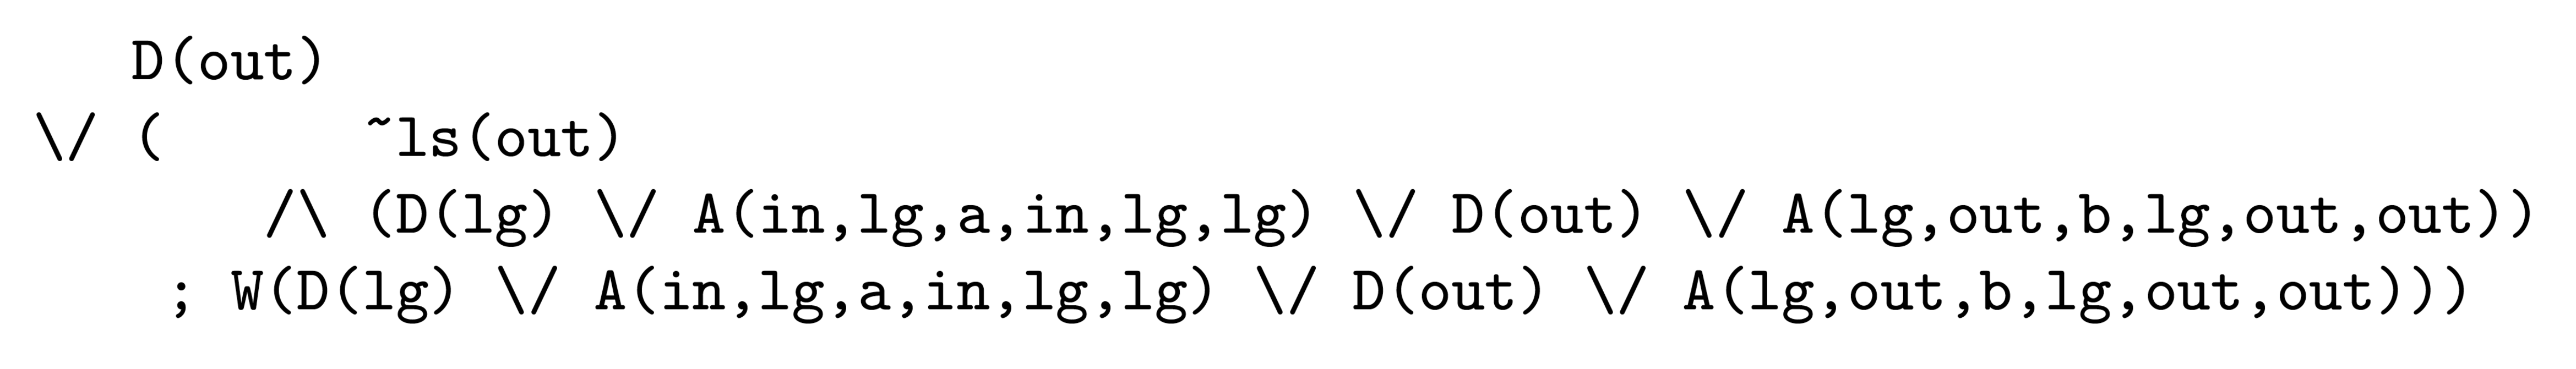
\includegraphics[scale=0.155]{pprint-xmpl.eps}

%{\small
%\begin{verbatim}
%    D(out)
% \/ (      ~ls(out)
%        /\ (D(lg) \/ A(in,lg,a,in,lg,lg) \/ D(out) \/ A(lg,out,b,lg,out,out))
%     ; W(D(lg) \/ A(in,lg,a,in,lg,lg) \/ D(out) \/ A(lg,out,b,lg,out,out)))
%\end{verbatim}
%}
\noindent
The top-level structure of this is
\[D(out) \lor ( (\lnot ls(out) \land \dots) ; W(\dots) )\]

\noindent
The pretty printing support can be found in \texttt{PrettyPrint.lhs},
which was written from scratch, but inspired by writings of
Hughes\cite{HughesJohn1995c} and Wadler\cite{wadler-pp}
on the subject.

In addition to the layout management aspects of pretty-printing
as just illustrated above,
there is also a need for a support for shorthand notations,
in order to ensure that predicates are more readable.
This particularly arises when set notation is in heavy use.
We illustrate this in Sect.\ref{sec:Expressions}.

\subsection{Dictionaries}\label{ssec:dict}

The approach taken is to implement a dictionary that maps names
to entries that supply extra information.
The names can be those of expression or predicate composites,
or correspond to variables, and a few other features of note.
All of the main calculator functions are driven by this
dictionary,
and the correct definition of dictionary entries
is the primary way for users to set up calculations.

%The standard approach is that the calculator
%will seek information regarding some name that is
%currently of interest.
%It will perform a dictionary lookup which can result
%in either failure, for which a suitable default action will be used,
%or success, in which case the dictionary entry will supply
%information to guide the required name-specific behaviour.
%
%There are four kinds of dictionary entries,
%one each for expressions and predicates,
%one for laws of various kinds,
%and one for alphabet handling.
%We will discuss each kind in turn,
%but leave examples of their use until Sect.\ref{sec:Theorising}.





\subsection{Impementation Overview}

The UTP Calculator is implemented as a series
of Haskell modules,
which are broken into two groups:
\begin{description}
  \item[Infrastructure]
    are modules that implement the calculator mechanics,
    pretty-printing, etc.
    These include \texttt{PrettyPrint},
    and all modules with names starting with \texttt{Calc}.
  \item[Builtin Theories]
    are pre-defined theory modules that cover standard logic,
    whose names start with \texttt{Std}, and modules that cover ``standard''
    UTP, whose names start with \texttt{StdUTP}.
    These theory modules typically come in threes, covering
    \texttt{Predicates}, \texttt{Precedences} and \texttt{Laws}.
\end{description}
All the code described here is available online
at
\\\url{https://bitbucket.org/andrewbutterfield/utp-calculator.git}
as Literate Haskell Script files (\texttt{.lhs})
in the \texttt{src} sub-directory.

\subsubsection{Display Convention}

In the rest of this paper, code that is part of the underlying
calculator infrastructure is shown as a simple verbatim display, thus:
\begin{verbatim}
underlying UTPCalc code
\end{verbatim}
while code supplied by the user to set it up for a particular
theory under investigation is shown enclosed in horizontal lines:
\begin{code}
user-supplied theory customisation code
\end{code}
